\subsubsection{Calculating Tu and Tg}



\subsubsection{Generating Hudzovic lookup curves}

As previously discussed, the Hudzovic method approximates the step response of a
plant using a PTn element, defined as

\begin{equation}
    G(s) = y_0 + K_s \prod_{k=1}^{n} \frac{1}{1+s \cdot T_k(r)} \textrm{\hspace{4mm}where\hspace{4mm}} T_k(r) = \frac{T}{1 - (k-1)r} \textrm{\hspace{4mm}and\hspace{4mm}} K_s = \frac{xa(\infty)}{xeo}
    \label{eq:hudzovic}
\end{equation}

where $0 \le r \leq \frac{1}{n-1}$.

That is, $G(s)$ is a series of multiplications of PT1 elements with varying time
constants $T_k$, scale factor $K_s$ and offset $y_0$:

\begin{equation}
    G(s) = y_0 + K_s \frac{1}{\left(1+s\cdot T_1\right)}\cdot\frac{1}{\left(1+s\cdot T_2\right)}\ldots\frac{1}{\left(1+s\cdot T_n\right)}
\end{equation}

Rather  than individually having to find the time constants $T_1\ldots  T_n$,  a
function $T_k(r)$ is instead  defined. The problem, thus, is to find appropriate
values for $n$, $T$ and  $r$  such that $G(s)$ approximates the step function of
the  given  plant as closely as possible. More specifically, $g_{T_u/T_g}$  must
equal    $plant_{T_u/T_g}$,    where     $g(t)$    is    the    step    response
$\mathscr{L}^{-1}\{\frac{G(s)}{s}\}$.

Unfortunately,  it  is not possible to directly calculate appropriate values for
$n$,  $T$  and  $r$,  as there are too many  unknowns.  However,  what  equation
\ref{eq:hudzovic} allows us to do now  is  calculate  an infinite number of step
responses  of  arbitrary  PTn  elements (while maintaining a constant number  of
input  arguments,  thanks to the function $T_k(r)$) and perform a reverse lookup
on those results to find the parameters $n$, $T$, $r$.

If we set $T=1$, $K_s=1$  and  $y_0=0$, we can use equation \ref{eq:hudzovic} to
calculate  a  series  of  transfer functions $G_{r,n}(s)$ (in  function  of  the
parameters   $r$  and  $n$),  calculate  their  time   domain   step   responses
$g_{r,n}(t)$,  and  calculate  $g_{T_u/T_g}$  and  $g_{1/T_g}$   for  each  step
response.

Thus, $g_{T_u/T_g}$ and $g_{1/T_g}$ can are both functions of $r$ and $n$:
\begin{align}
    g_{T_u/T_g} = g_{T_u/T_g}(r, n) \\
    g_{1/T_g}  =  g_{1/T_g}(r,n)
\end{align}
Visualising    this    data    yields    the     curves    seen    in    figures
\ref{fig:hudzovic:curves_tu_tg}        and       \ref{fig:hudzovic:curves_t_tg}.

Finding $n$ is now a simple matter of  computing $plant_{T_u/T_g}$ and comparing
the  result  to the Y axis in figure \ref{fig:hudzovic:curves_tu_tg} for  $r=0$.
Ideally, we'd  like  $n$  to  be as small as possible, so the following equation
must be satisfied.
\begin{equation}
    g_{T_u/T_g}(r, n)\lvert_{r=0} \hspace{2mm} \le \hspace{2mm} plant_{T_u/T_g}
\end{equation}

With the parameter $n$ defined, the next step is to find  the intersection point
of $g_{T_u/T_g}(r, n)$  with  the  horizontal  line  $plant_{T_u/T_g}$ in figure
\ref{fig:hudzovic:curves_tu_tg}. This will yield parameter $r$.

The last parameter, $T$,  can  finally  be  determined  by evaluating $T_g \cdot
g_{1/T_g}(r, n)$. Graphically, this equates to finding the intersection point of
the vertical line going through $r$ and the function $g_{1/T_g}(r, n)$ in figure
\ref{fig:hudzovic:curves_t_tg} and multiplying the result by $T_g$.

\begin{figure}
     \centering
     \begin{subfigure}[b]{0.8\textwidth}
         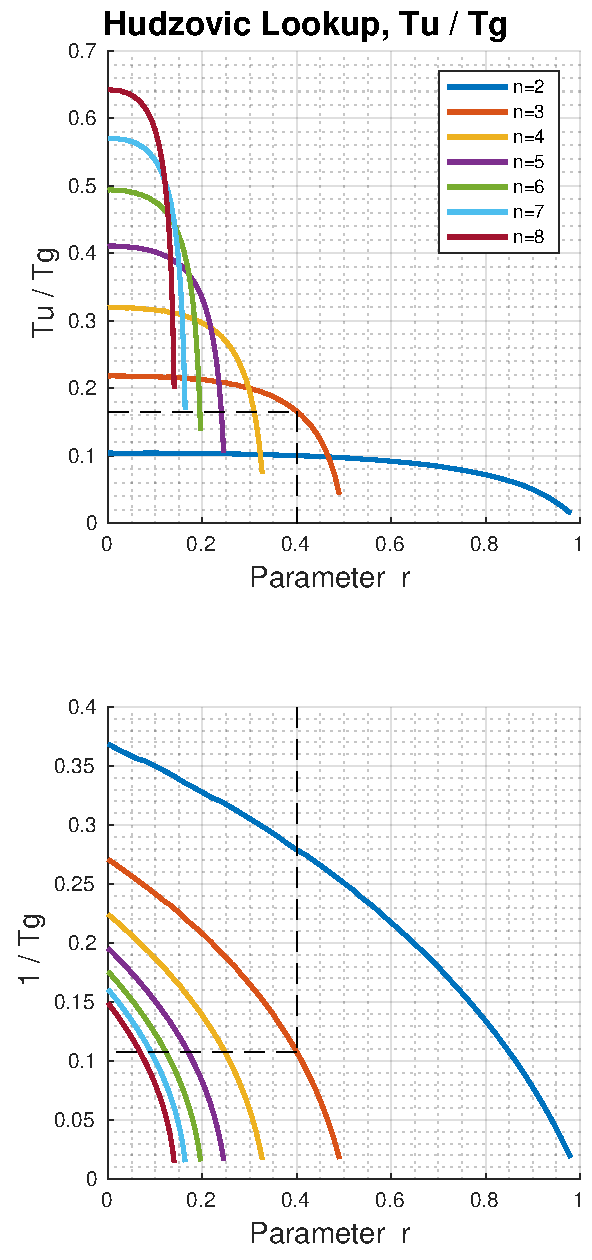
\includegraphics[width=1\linewidth]{images/hudzovic_curves_tu_tg}
         \caption{Tu/Tg in function of r and n}
         \label{fig:hudzovic:curves_tu_tg}
    \end{subfigure}
    \begin{subfigure}[b]{0.8\textwidth}
        \centering
        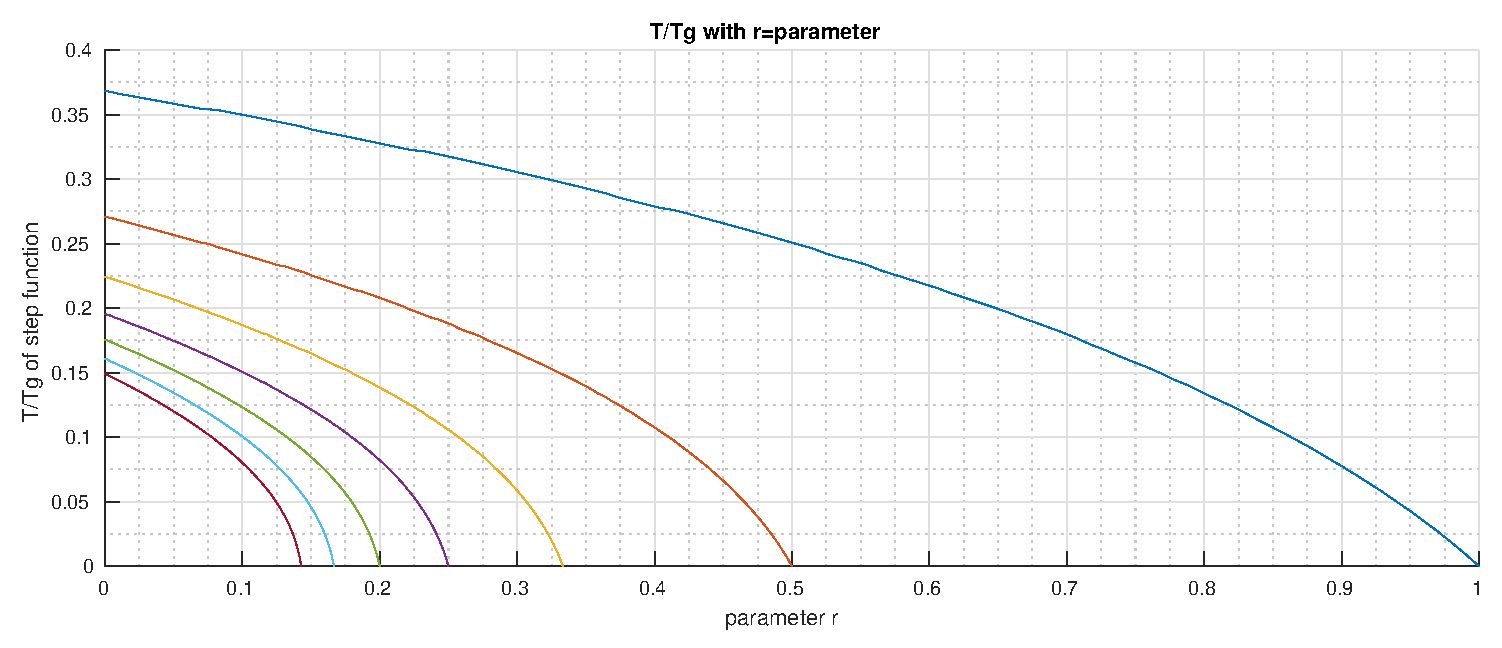
\includegraphics[width=1\linewidth]{images/hudzovic_curves_t_tg}
        \caption{T/Tg in function of r and n}
        \label{fig:hudzovic:curves_t_tg}
    \end{subfigure}
    \caption{Hudzovic lookup curves}
\end{figure}

